\chapter{LITERATURE REVIEW}

\section*{ }
To support this research, several relevant theories are required as references and conceptual foundations. This will help ensure the research is well-directed and aligned with existing scientific knowledge.
\vspace{1ex}

% \section{Robot Navigation System}
% A robot navigation system consists of two main components: (1) determining the robot's pose (position and orientation), and (2) determining the robot’s actions based on that information. Robot poses are generally classified as 2D or 3D. A 2D pose system uses three degrees of freedom (DoF): the x-axis, y-axis, and rotation around the z-axis. These three components are typically represented as \(x, y, \text{yaw}\).

\section{Odometry}
Odometry is an algorithm used to estimate how far a robot has traveled. In a 2D pose system, the robot’s movement is represented as \(x, y, \text{yaw}\). The simplest form of 2D odometry combines motor rotation data with orientation data from an Inertial Measurement Unit (IMU). By applying forward kinematics to this sensor data, the robot's pose can be estimated relative to its initial position \cite{ref_mas_marin}.

\section{Bicycle Model}
The bicycle model is a simplified mathematical representation of vehicle dynamics. It models a vehicle as a two-wheel system—one at the front and one at the rear—mimicking the dynamics of a bicycle. This model is widely used in vehicle control and trajectory planning due to its simplicity and ability to capture basic vehicle behavior \cite{rajamani2011vehicle}. In robotics and electrical engineering, the bicycle model is commonly used to develop navigation and motion control algorithms for autonomous ground vehicles.

\begin{equation}
	\begin{aligned}
		\delta_{\text{target}} &= \tan^{-1}\left( \frac{2 \cdot L \cdot \sin(\theta_{\text{direction}})}{D_{\text{lookahead}}} \right)
		\label{eq:bicycle_model_core}
	\end{aligned}		
\end{equation}

where \(\delta_{\text{target}}\) is the target steering angle, \(L\) is the distance between the front and rear wheels, \(\theta_{\text{direction}}\) is the heading angle, and \(D_{\text{lookahead}}\) is the lookahead distance.

\par
The main advantage of the bicycle model is its applicability in control and simulation algorithms such as PID, LQR, and MPC. Many autonomous vehicle systems use it as a foundational model for motion prediction and path following. For instance, it enables calculation of the optimal steering angle required for a vehicle to accurately and stably follow a predefined trajectory \cite{paden2016survey}.

\section{GNSS}
The Global Navigation Satellite System (GNSS) is a satellite-based system that provides highly accurate global information on position, velocity, and time. GNSS encompasses multiple satellite navigation systems, including GPS (USA), GLONASS (Russia), Galileo (EU), and BeiDou (China), which can function independently or in combination \cite{misra2006gps}. In electrical engineering and robotics, GNSS plays a critical role in navigation and positioning, particularly for mobile robots operating in open environments.

\par
GNSS operates by measuring the time required for satellite signals to reach a receiver. A GNSS receiver can compute a 3D position using signals from at least four satellites. Techniques such as Differential GNSS (DGNSS) and Real-Time Kinematic (RTK) improve accuracy by applying corrections from fixed reference stations \cite{kaplan2017understanding}. These techniques are especially beneficial in applications like precision agriculture, drones, and autonomous vehicles.

\par
GNSS can be integrated with other systems such as Inertial Navigation Systems (INS) to enhance reliability in environments where satellite signals are blocked, such as under tree canopies or between buildings \cite{grewal2013gnss}. Integration with sensors like IMUs, LiDARs, and cameras also enhances performance in SLAM systems.

\par
Beyond navigation, GNSS contributes to control systems, trajectory planning, and multi-robot coordination. With ongoing advances in satellite infrastructure and error correction algorithms, GNSS remains a cornerstone for the development of efficient and precise outdoor robotic systems.

\section{Kalman Filter}
The Kalman Filter is a powerful linear estimation algorithm used to predict and update the state of dynamic systems based on noisy sensor data. Introduced by Rudolf E. Kalman in 1960, it enables accurate real-time estimation of variables such as position and velocity \cite{kalman1960new}. In robotics and control systems, the Kalman Filter is instrumental in fusing data from multiple sensors such as GNSS, IMUs, and wheel encoders.

\par
The algorithm consists of two stages: prediction and update. During the prediction stage, the system state is estimated using a motion model. In the update stage, the estimate is refined based on new sensor measurements. This iterative process results in increasingly accurate state estimations \cite{welch2006kalman}.

\section{SLAM}
Simultaneous Localization and Mapping (SLAM) is a foundational technology in autonomous robotics. It allows a robot to construct a map of an unknown environment while simultaneously estimating its own position within that map. SLAM is particularly valuable in GPS-denied environments and is widely used in autonomous vehicles, drones, and mobile robots \cite{cadena2016past}.

\section{Graph-Based SLAM}
SLAM techniques can be divided into two broad categories: filter-based SLAM (e.g., Extended Kalman Filter SLAM) and graph-based SLAM. In filter-based SLAM, the robot's pose and landmark positions are treated as stochastic variables updated recursively. In contrast, graph-based SLAM builds a graph where nodes represent robot poses and landmarks, and edges represent spatial constraints derived from sensor observations \cite{thrun2005probabilistic}.


\begin{figure}[H]
	\centering
	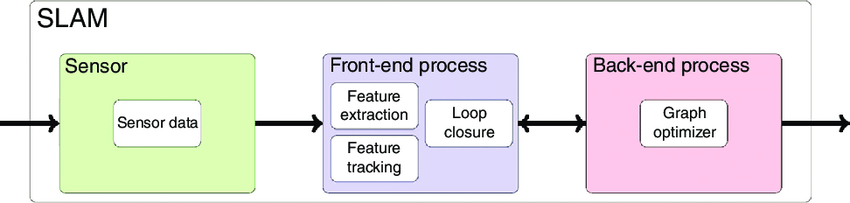
\includegraphics[width=\linewidth]{../konten/gb_slam.png}
	\caption{Basic Graph-Based SLAM Architecture \cite{ref_gb_slam}}
	\label{fig:basic_graph_based_slam}
\end{figure} 

There are three main process that can be seen from figure \ref{fig:basic_graph_based_slam}: The first process is sensor data, it means like acquiring data from sensors such as cameras, LIDAR, or IMU. The second process is front end process, The front end process is responsible for extracting features from the sensor data and finding a loop closure. The last process is back end process, the back end process is responsible for optimizing the graph to find the best estimate of the robot's trajectory and the map of the environment \cite{ref_gb_slam}.

\par
The optimization in Graph-based SLAM can be efficiently implemented using frameworks like GTSAM (Georgia Tech Smoothing and Mapping), a C++ library that applies nonlinear optimization over factor graphs. Factor graphs represent probabilistic relationships among variables such as odometry, landmarks, and sensor observations, and allow for efficient optimization of robot trajectories \cite{ref_gtsam}.

\section{RTAB-Map}
RTAB-Map (Real-Time Appearance-Based Mapping) is a graph-based SLAM framework designed for real-time applications in robotics. It integrates various sensors, including cameras, LIDARs, GPS, IMUs, and Odometry, to build a map of the environment while simultaneously localizing the robot within that map. RTAB-Map is particularly effective in large-scale environments and can handle loop closures and dynamic changes in the environment \cite{ref_rtabmap}.

\section{Stereo Depth Camera}
A stereo depth camera is a vision-based depth sensing system that uses two calibrated cameras to capture two images from slightly different perspectives—similar to human binocular vision. By analyzing the disparity between corresponding points in the image pair, the system calculates the depth or distance of objects \cite{scharstein2002taxonomy}.

\par
Stereo cameras are widely used in robotics due to their ability to generate real-time depth maps without requiring active sensors like LiDAR. They are especially useful in lightweight and power-efficient robotic platforms such as drones and small autonomous vehicles \cite{khoshelham2012accuracy}.

\section{Machine Learning}
Machine learning (ML) is a subset of artificial intelligence that focuses on creating algorithms capable of learning from data and improving performance without being explicitly programmed \cite{mitchell1997machine}. In robotics and electrical engineering, ML is essential for building intelligent systems that can recognize patterns, make decisions, and adapt to changing environments.

\par
ML methods are typically categorized into three types: supervised learning, unsupervised learning, and reinforcement learning \cite{goodfellow2016deep}. Supervised learning uses labeled datasets for tasks like classification and regression. Unsupervised learning deals with unlabeled data for clustering or dimensionality reduction. Reinforcement learning enables systems to learn optimal behaviors through reward-based interactions with the environment.

\par
A key ML technique in robotic perception is semantic segmentation, which classifies each pixel in an image into predefined categories. This technique is widely used for road detection, scene understanding, and navigation.

\section{Semantic Segmentation}

Fast-SCNN (Fast Semantic Segmentation Convolutional Neural Network) was designed for real-time performance on resource-constrained devices, making it ideal for embedded systems like autonomous vehicles. It combines a lightweight encoder-decoder structure with efficient components such as depthwise separable convolutions and a streamlined feature fusion strategy. These design choices enable Fast-SCNN to achieve a good balance between accuracy and speed, ensuring that road segmentation can be performed in real time without requiring GPU-level hardware.

\begin{figure}[H]
	\centering
	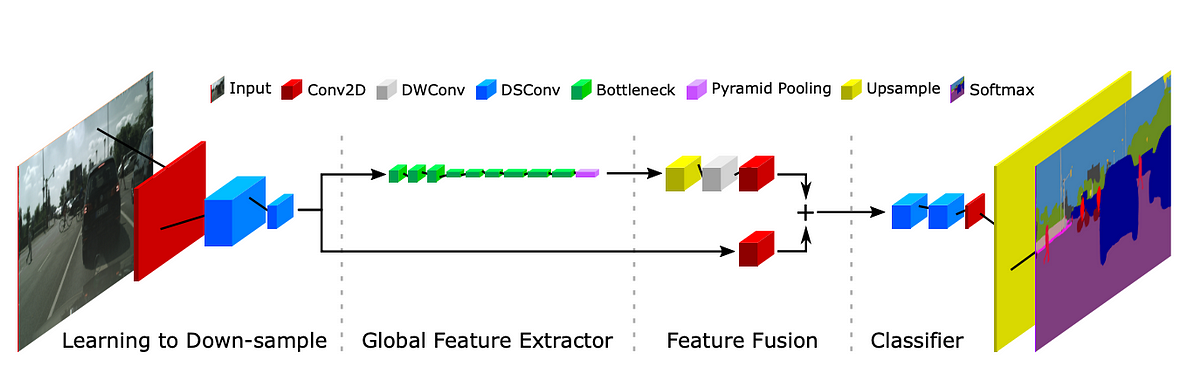
\includegraphics[width=\linewidth]{../konten/fast_scnn.png}
	\caption{Fast SCNN Architecture \cite{ref_fast_scnn}}
	\label{fig:fast_scnn_architecture}
\end{figure} 

Fast-SCNN consists of four main modules: Learning to Downsample, Global Feature Extractor, Feature Fusion Module, and Classifier. The network first reduces the spatial dimensions of the input image while increasing feature richness, then extracts global context features and fuses them with fine spatial details. This fused representation is finally classified at the pixel level to distinguish road and non-road areas. In the Icar system, this segmented output supports safe navigation by identifying drivable regions based on real-time camera input \cite{ref_fast_scnn}.

\section{Iterative Closest Point (ICP)}
Iterative Closest Point (ICP) is a widely used algorithm in known-map localization that aligns two 3D point clouds: one from the robot's current observation and one from a reference map \cite{ref_icp}. The output is a transformation matrix that minimizes the difference between the two point sets.

\par
The ICP algorithm operates in three main steps: first, for each point in the input point cloud, it finds the nearest point in the reference point cloud (using nearest-neighbor search). Second, it calculates the centroids (center of mass) of both point clouds and aligns them via translation. Third, it applies rotation—typically using Singular Value Decomposition (SVD)—to best align the clouds.

\par
These steps are repeated iteratively until convergence, defined by either reaching a maximum number of iterations or achieving a sufficiently low alignment error. The final result is the transformation matrix that aligns the current observation with the reference map, enabling accurate pose estimation.

\section{Binary Robust invariant scalable keypoints (BRISK)}
BRISK Binary Robust invariant scalable keypoints is a real-time feature method that combines a novel scale-space FAST detector with a binary bit-string descriptor built from intensity-comparison sampling. Keypoints are detected across scales via a FAST-based pyramid, then each is described by a 512-bit string derived from Gaussian-smoothed intensity comparisons on concentric sampling rings, with an orientation normalization step for rotation invariance. Evaluated on standard benchmarks, BRISK matches the accuracy of heavy float descriptors like SURF and SIFT while running up to an order of magnitude faster, making it highly suited for resource-constrained, real-time vision applications \cite{ref_brisk}.